\documentclass[border=6pt]{standalone}
\usepackage{tikz}
\usetikzlibrary{arrows.meta,positioning,calc,shapes.geometric,fit,backgrounds,patterns,matrix,decorations.pathreplacing}
\begin{document}
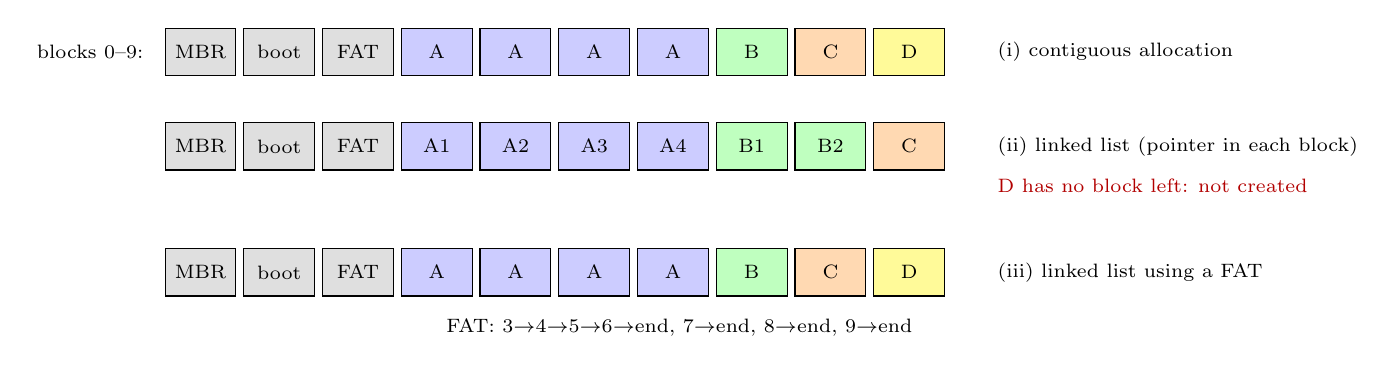
\begin{tikzpicture}[>=Stealth,font=\small]
\tikzstyle{b}=[draw,minimum width=0.9cm,minimum height=0.6cm,font=\scriptsize]
\foreach \i/\n in {0/MBR,1/boot,2/FAT} \node[b,fill=gray!25] at (\i,0) {\n};
\node[font=\scriptsize,anchor=east] at (-0.6,0) {blocks 0--9:};
\node[font=\scriptsize,anchor=west] at (10,-0.0) {(i) contiguous allocation};
\foreach \i/\n/\c in {3/A/blue!20,4/A/blue!20,5/A/blue!20,6/A/blue!20,7/B/green!25,8/C/orange!30,9/D/yellow!40} \node[b,fill=\c] at (\i,0) {\n};
\foreach \i/\n in {0/MBR,1/boot,2/FAT} \node[b,fill=gray!25] at (\i,-1.2) {\n};
\node[font=\scriptsize,anchor=west] at (10,-1.2) {(ii) linked list (pointer in each block)};
\foreach \i/\n/\c in {3/A1/blue!20,4/A2/blue!20,5/A3/blue!20,6/A4/blue!20,7/B1/green!25,8/B2/green!25,9/C/orange!30} \node[b,fill=\c] at (\i,-1.2) {\n};
\node[font=\scriptsize,red!70!black,anchor=west] at (10,-1.7) {D has no block left: not created};
\foreach \i/\n in {0/MBR,1/boot,2/FAT} \node[b,fill=gray!25] at (\i,-2.8) {\n};
\node[font=\scriptsize,anchor=west] at (10,-2.8) {(iii) linked list using a FAT};
\foreach \i/\n/\c in {3/A/blue!20,4/A/blue!20,5/A/blue!20,6/A/blue!20,7/B/green!25,8/C/orange!30,9/D/yellow!40} \node[b,fill=\c] at (\i,-2.8) {\n};
\node[font=\scriptsize,anchor=west] at (3,-3.5) {FAT: 3$\to$4$\to$5$\to$6$\to$end, 7$\to$end, 8$\to$end, 9$\to$end};
\end{tikzpicture}
\end{document}
